% Progress Report Document
\documentclass[progress]{cmpreport}
\makeatletter
\input{t1pcr.fd}
\makeatother
\setlength{\footnotesep}{3ex}
\title{\Codex: A Website and Progressive Web App in Node.js \& React for table-top role-playing games}
\author{Christopher Alastair Irvine}
\registration{100036248}
\supervisor{Dr Katharina Huber}
\ccode{CMP-6013Y}
\summary{This document is the Progress Report for Codex}
\acknowledgements{
	I would like to thank Dr Katharina Huber for taking on the supervision of this project, 
	and guiding me towards greatness. Additionally I would like to thank Wizards of the Coast 
	for their generosity and kindness in allowing the use of their Intellectual Property for this project.
}
\usepackage{rotating}
\usepackage{amsmath}
\usepackage{lscape}
\usepackage{hhline}
\newcommand{\ueacmp}{UEA School of Computing Sciences}
\newcommand{\WotC}{Wizards of the Coast}
\newcommand{\dnd}{D\&D}
\newcommand{\sem}{Software Engineering Model}
\newcommand{\sems}{Software Engineering Models}
\newcommand{\Codex}{\textsc{Codex}}
\newcommand{\AgileSolo}{\emph{Agile Solo}}
% EOF Preamble and Macros
	
% BOF Document
\begin{document}
	% BOF Introduction
	\section{Introduction} \label{sec:intro}
	% Introduction to the project:
	Before we can gain an understanding of the progress of \Codex, we must first understand the material that \Codex deals with. Namely Dungeons and Dragons (\dnd). \dnd is a deep and complex game, but at its core it is simple, and for the purposes of this document we only need to understand a handful of principles about the game that show why \Codex \ is being developed. These principles are: \dnd \ is random by nature, \dnd \ is based off simple mathematics that is easily modelled and \dnd \ cannot survive without a healthy population of \emph{Dungeon Masters} (DM). But first, what is \dnd \ and what is needed to play it? 
	
	\subsection{What is \dnd?}
	\dnd is a popular table-top role-playing game. Where a group of players (known as the \emph{Party}), must find a way past a series of challenges (called the \emph{Campaign}), created by the Dungeon Master (\emph{DM}), as they explore the world that the DM has created. Almost everything that happens during a Campaign is determined by a series of dice rolls that decide if an attack hits an enemy or if a lock is picked open. Sometimes even something as getting from point A to point B in the world can go awry from a set of unfortunate die rolls.
	
	\begin{figure}[h] 
		\begin{subfigure}{0.5\textwidth}
			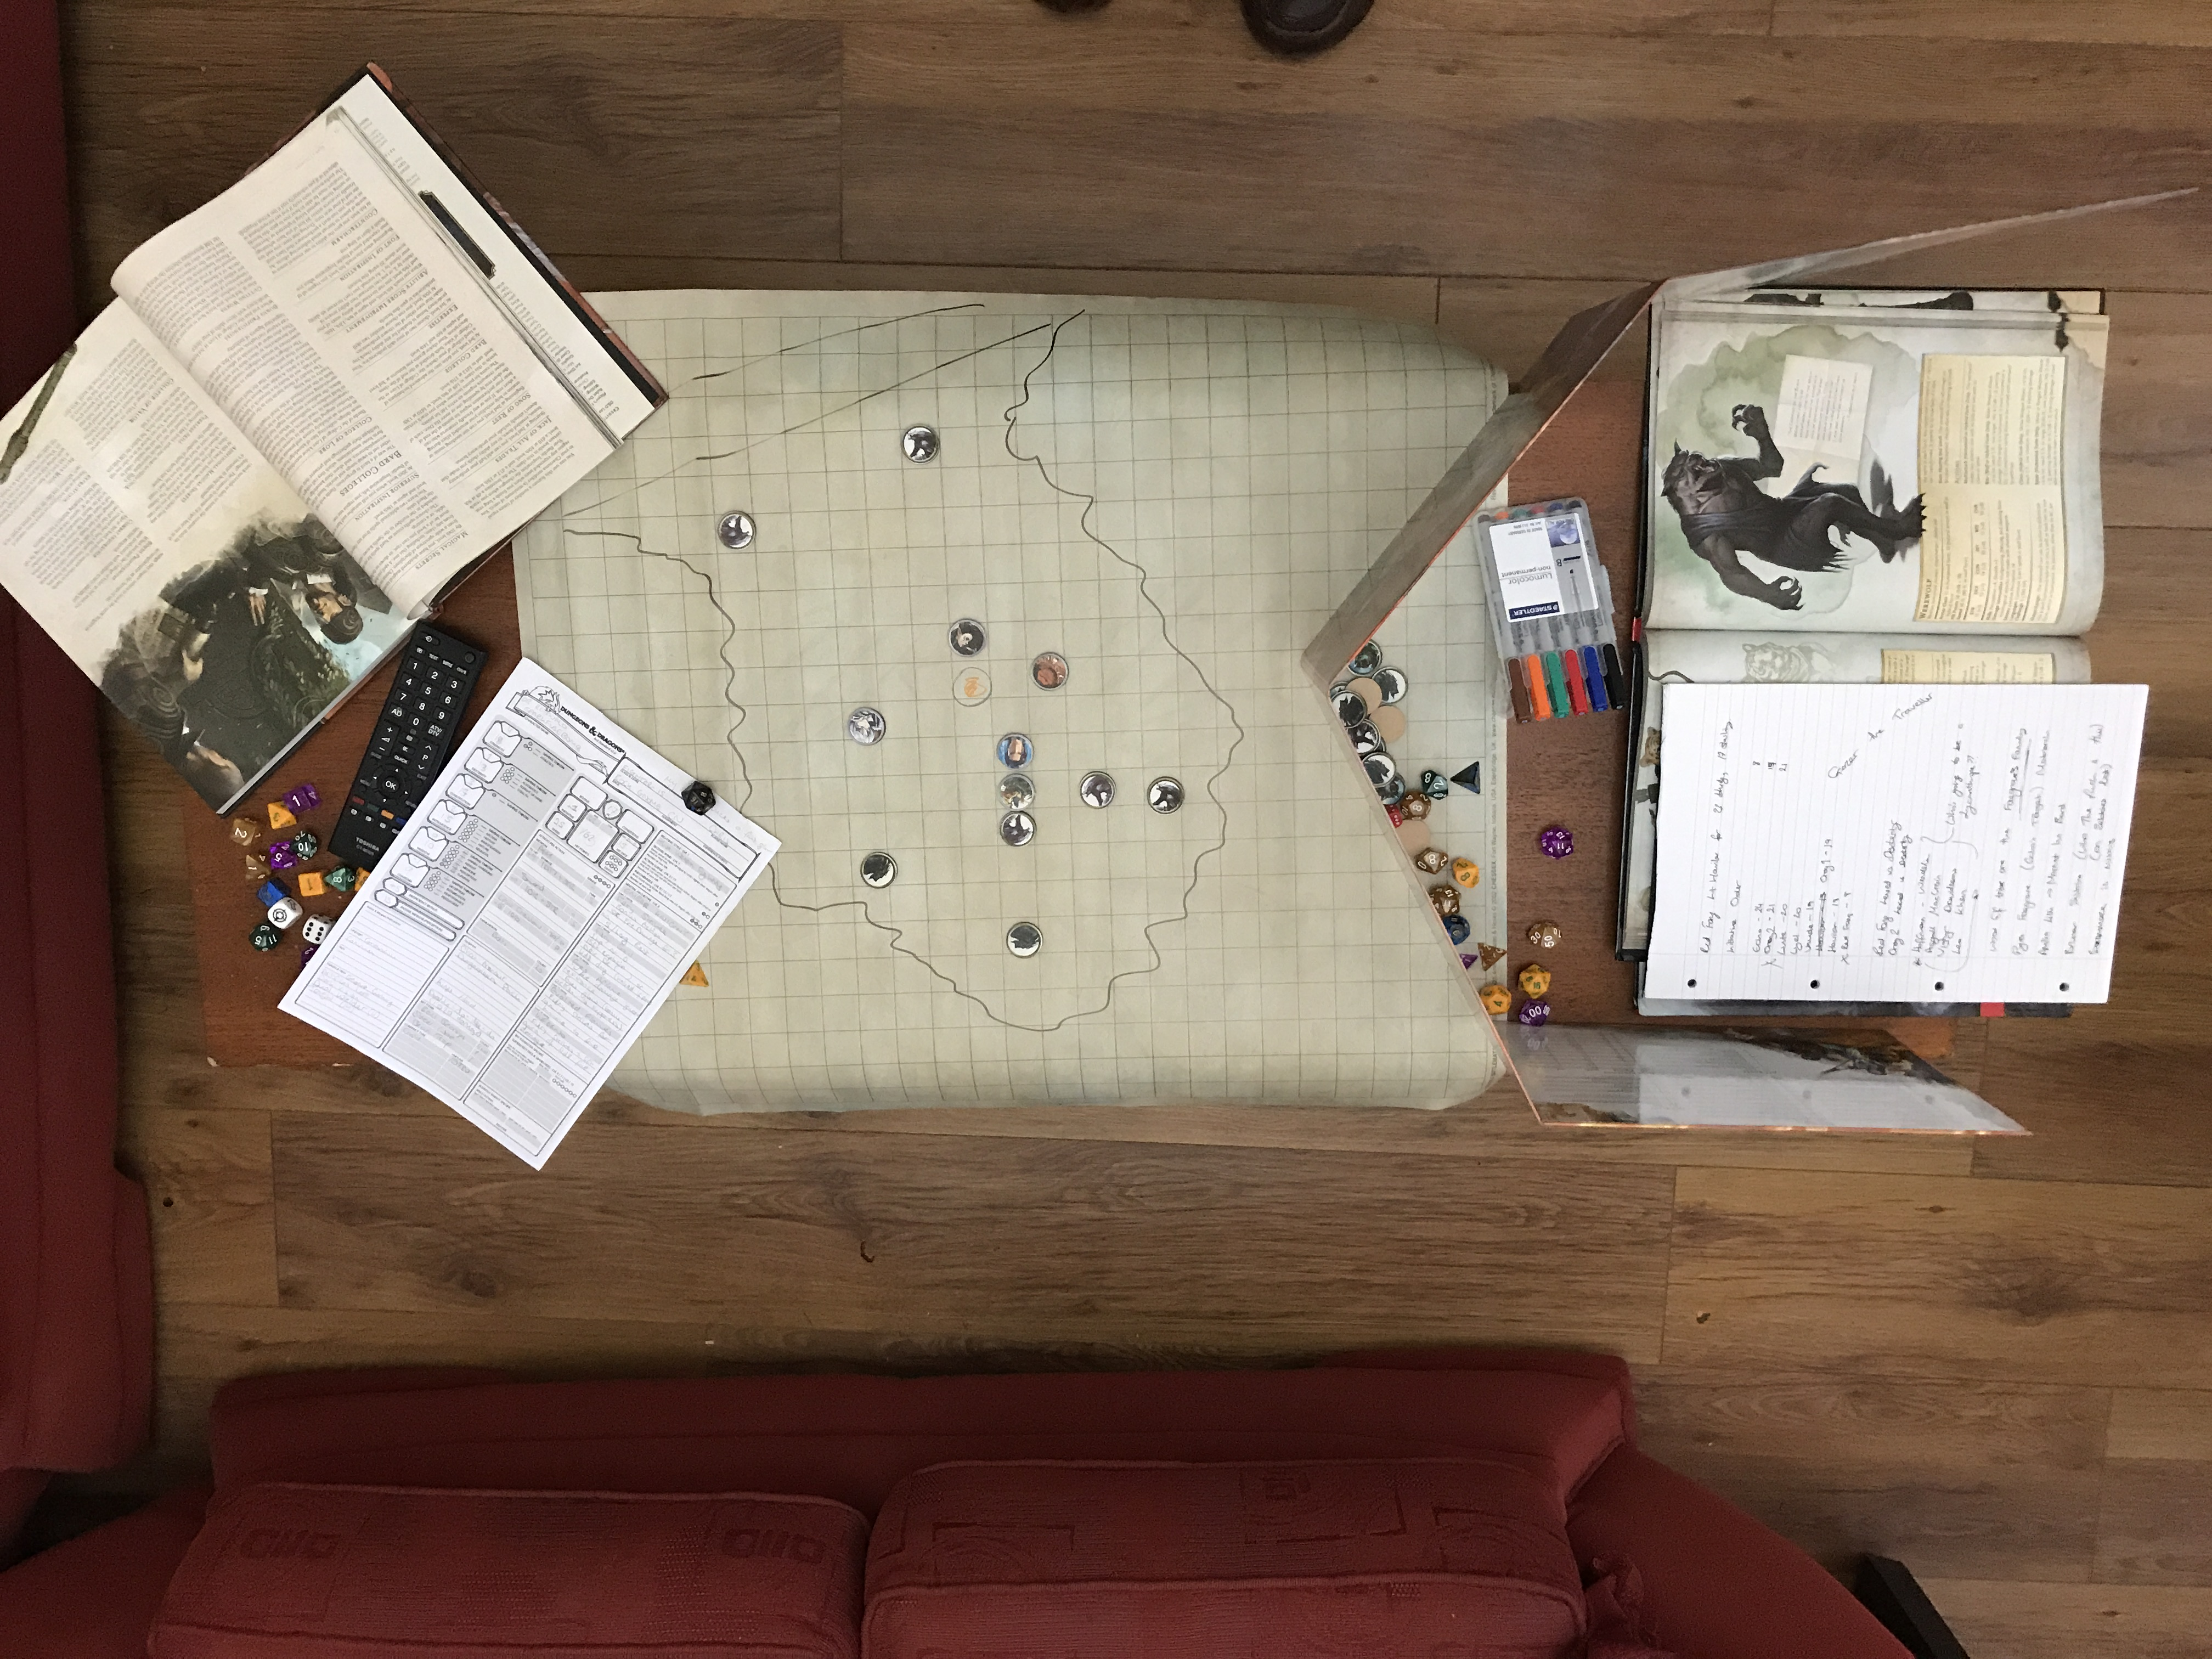
\includegraphics[width=1\linewidth, height=5cm, angle=180]{DnD_Live.jpg}
			\caption{A typical \dnd set up} 
			\label{DnDLive}
		\end{subfigure}
		\begin{subfigure}{0.5\textwidth}
			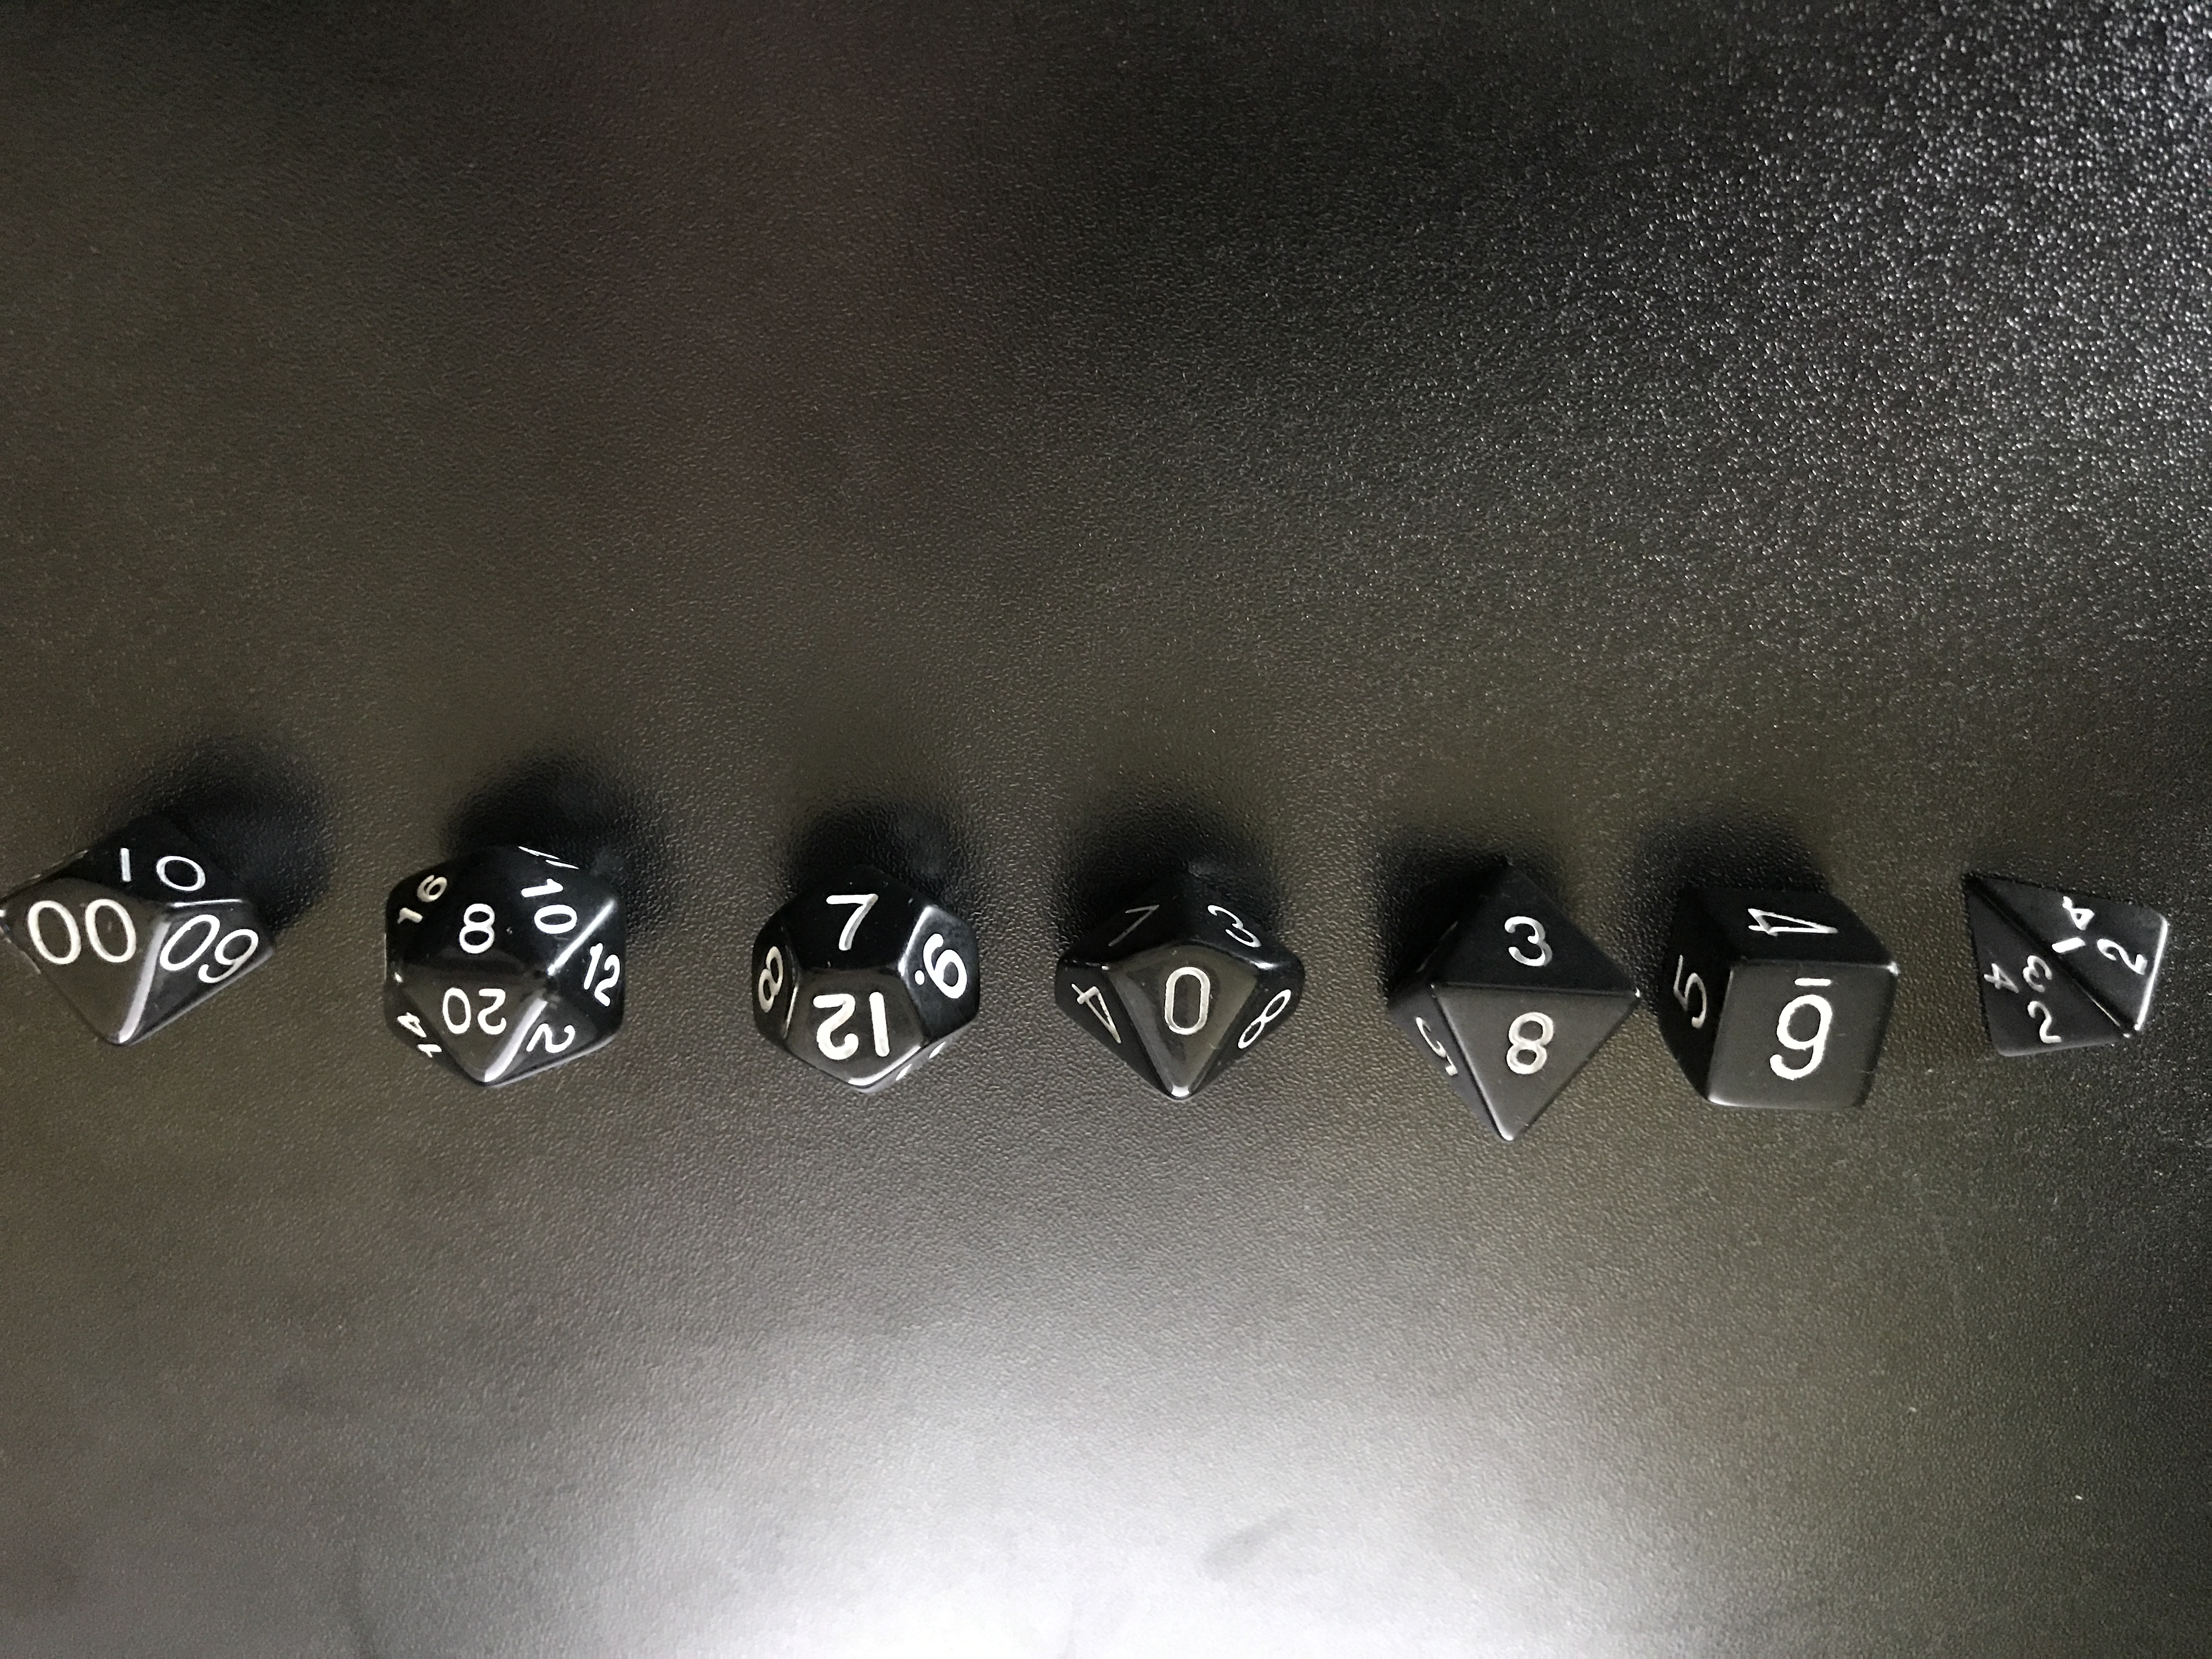
\includegraphics[width=1\linewidth, height=5cm, angle=180]{DnD_Dice.jpg}
			\caption{The Die necessary to play \dnd} 
			\label{DnDDice}
		\end{subfigure}
		\caption{These two figures show the typical equipment for a \dnd \ game}
		\label{DnDEquipmentExample}
	\end{figure}

	Only a limited amount of equipment is needed to play \dnd; a set of die, character sheet, paper and pencil. Each group will also need the \emph{core books} (Player's Handbook, Dungeon Master's Guide and Monster Manual) between them. Optional equipment include (but is not limited to) a battle map, tokens and a DM screen. This equipment can be seen in Figure \ref{DnDEquipmentExample}. From left to right in Figure \ref{DnDEquipmentExample} (a), we can see one of the core books, a pad of paper, a collection of the various die, DM screen, battle mat with tokens, a character sheet, some more die and another of the core books. Figure \ref{DnDEquipmentExample} (b) shows the die used in \dnd \ which are; 4, 6, 8, 10, 12, 20 and 100-sided. The die are denoted as \emph{dXXX}, X being the number of sides to that die. 

	\subsection{The Dungeon Master}
	As explained above, the DM creates the world in front of the party and controls the narrative of the Campaign. This narrative could come from a purchased supplementary book written by \WotC (the company that make \dnd) or the DM could create the story themselves. Either way the DM needs to know both the world and the story they want to tell inside out. Even if then a DM needs to have excellent improvisational skills for when the Party does something unexpected. The challenge of playing the role of DM is to know what you want to happen next and guide the Party to that event without the Party feeling forced into it. It is that challenge that makes the role of DM hard work and fun at the same time. It is not uncommon for a DM to have a couple of folders full to the brim with notes \citep{GMTips}. Fulfilling the role of the DM is like being a mastermind, pulling strings from the shadows, whilst trying to look after a large litter of over-active puppies. 

	\subsection{\dnd \ is random}
	Due to the importance placed on the result of die rolls, anything and everything can go wrong. Whilst the overarching story tends to stay the same the small details can change multiple times over the same session. This can make preparing content for the Party a living nightmare for a DM. Many a DM have found themselves having hours of preparation work wasted because of the result of a die roll or a decision made by the Party. But this is no one's fault. The Party do not know what is happening next and the DM can only react to the actions of the Party. It is the chaotic nature of \dnd. 
	
	\subsection{Mathematics of \dnd}
	As previously stated, almost everything that happens during a Campaign is decided by die rolls. However the Party (and the \emph{characters} they encounter) do have a small degree of control over their actions. Each character in \dnd \ has a set of \emph{ability scores} that make them unique, each score having a value of 0 to 20 (unless an item changes that) \citep{PlayerHandbook}. These ability scores are translated into \emph{ability modifiers}, which, for better or worse, affect the outcome of the die roll. If a character is particularly skilled in a task they are said to be \emph{Proficient} in it, further adjusting the outcome of a die roll. With the exception of damage rolls, the d20 die is used to make decisions in \dnd. Albeit with some minor variations, die rolls in \dnd \ 5\textsuperscript{th} Edition follow this formula:
	\begin{gather*}
		d20 + ability \ score + proficiency = result \\
		For \ example: \\
		15 + 4 + 2 = 21
	\end{gather*}
	However, as far as \Codex is concerned, the Party and DM will perform these calculations for themselves as its part of the fun of the game. Attack rolls, damage rolls and ability checks will be held out width \Codex. The mathematics that \Codex will handle is the calculation of Ability Modifiers:
	\begin{gather*}
		\frac{(ability \ score - 10)}{2} \ (rounded \ down)
	\end{gather*}
	In addition to the tracking of each character's \emph{hit points} during combat. Which is a simple addition or subtraction depending on whether a character took damage or gained healing.	

	% What is Codex? 
	% What is the purpose? 
	% What problems does Codex solve? 
	% How will it solve them?
	\subsection{What is \Codex?} \label{subsec:WIC}
	Now we have an understanding of \dnd, we can now understand the purpose of \Codex \ and what problems \Codex seeks to address. \Codex \ is a Software Engineering Project that aims to engineer a Web-App built in ReactJS and Node.JS technologies. The functionality of which is to:
	\begin{itemize}
		\item Assist the DM with the preparation of \dnd \ content.
		\item Track the Combat Statistics of each character during Encounter.
		\item Give the Party access to the rich lore of the world they play in.
	\end{itemize}
	\Codex \ is developed using the Agile Solo methodology \citep{AgileSolo}. Agile Solo provides \Codex \ with a structures environment of regular deadlines to ensure that the project stays on track. 
	
	ReactJS was chosen because of the ability to rapidly built and prototype User Interfaces (UI) across multiple platforms \citep{ReactJSOfficial}. Node.JS will handle the communication between \Codex \ and the corresponding database \citep{NodejsOfficial}. Both of these technologies follow the basic Web-App Architecture laid out in Figure \ref{Web-App-Arch}.
	\begin{figure}
		\centering
		\fbox{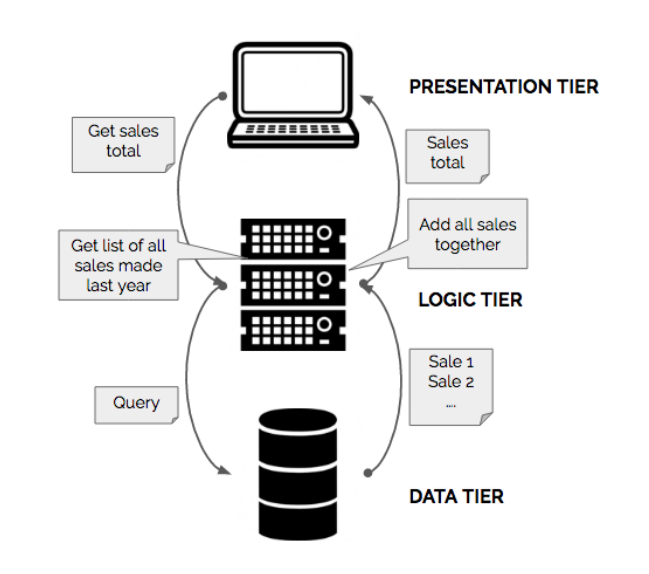
\includegraphics[width=0.5\textwidth]{Basic_Web_App_Architecture.PNG}} 
		\caption{Overview of a three-tier application and its dependencies \citep{SecurityWebApps}} \label{Web-App-Arch}
	\end{figure}
	
	\section{\Codex \ Design}
	% Cherry pick sections from the Design Document, summarising how Codex is designed and why I made those choices.
	In this section, the Design of \Codex \ that has been developed over the last three months will be critiqued and an overview of the critical elements of the Design will be presented. The development of the \Codex \ Design followed the Agile Solo weekly sprint formula. This was achieved by the single developer working on \Codex \ asking themselves a series of questions and recording their answers at the end of each week. Every two weeks the developer would aim to meet with their supervisor to ensure that \Codex \ was on track and any issues were being addressed. Trello was used to organise and manage the remaining tasks of the Design \citep{trello}.
	
	\begin{figure}[h]
		\centering
		\fbox{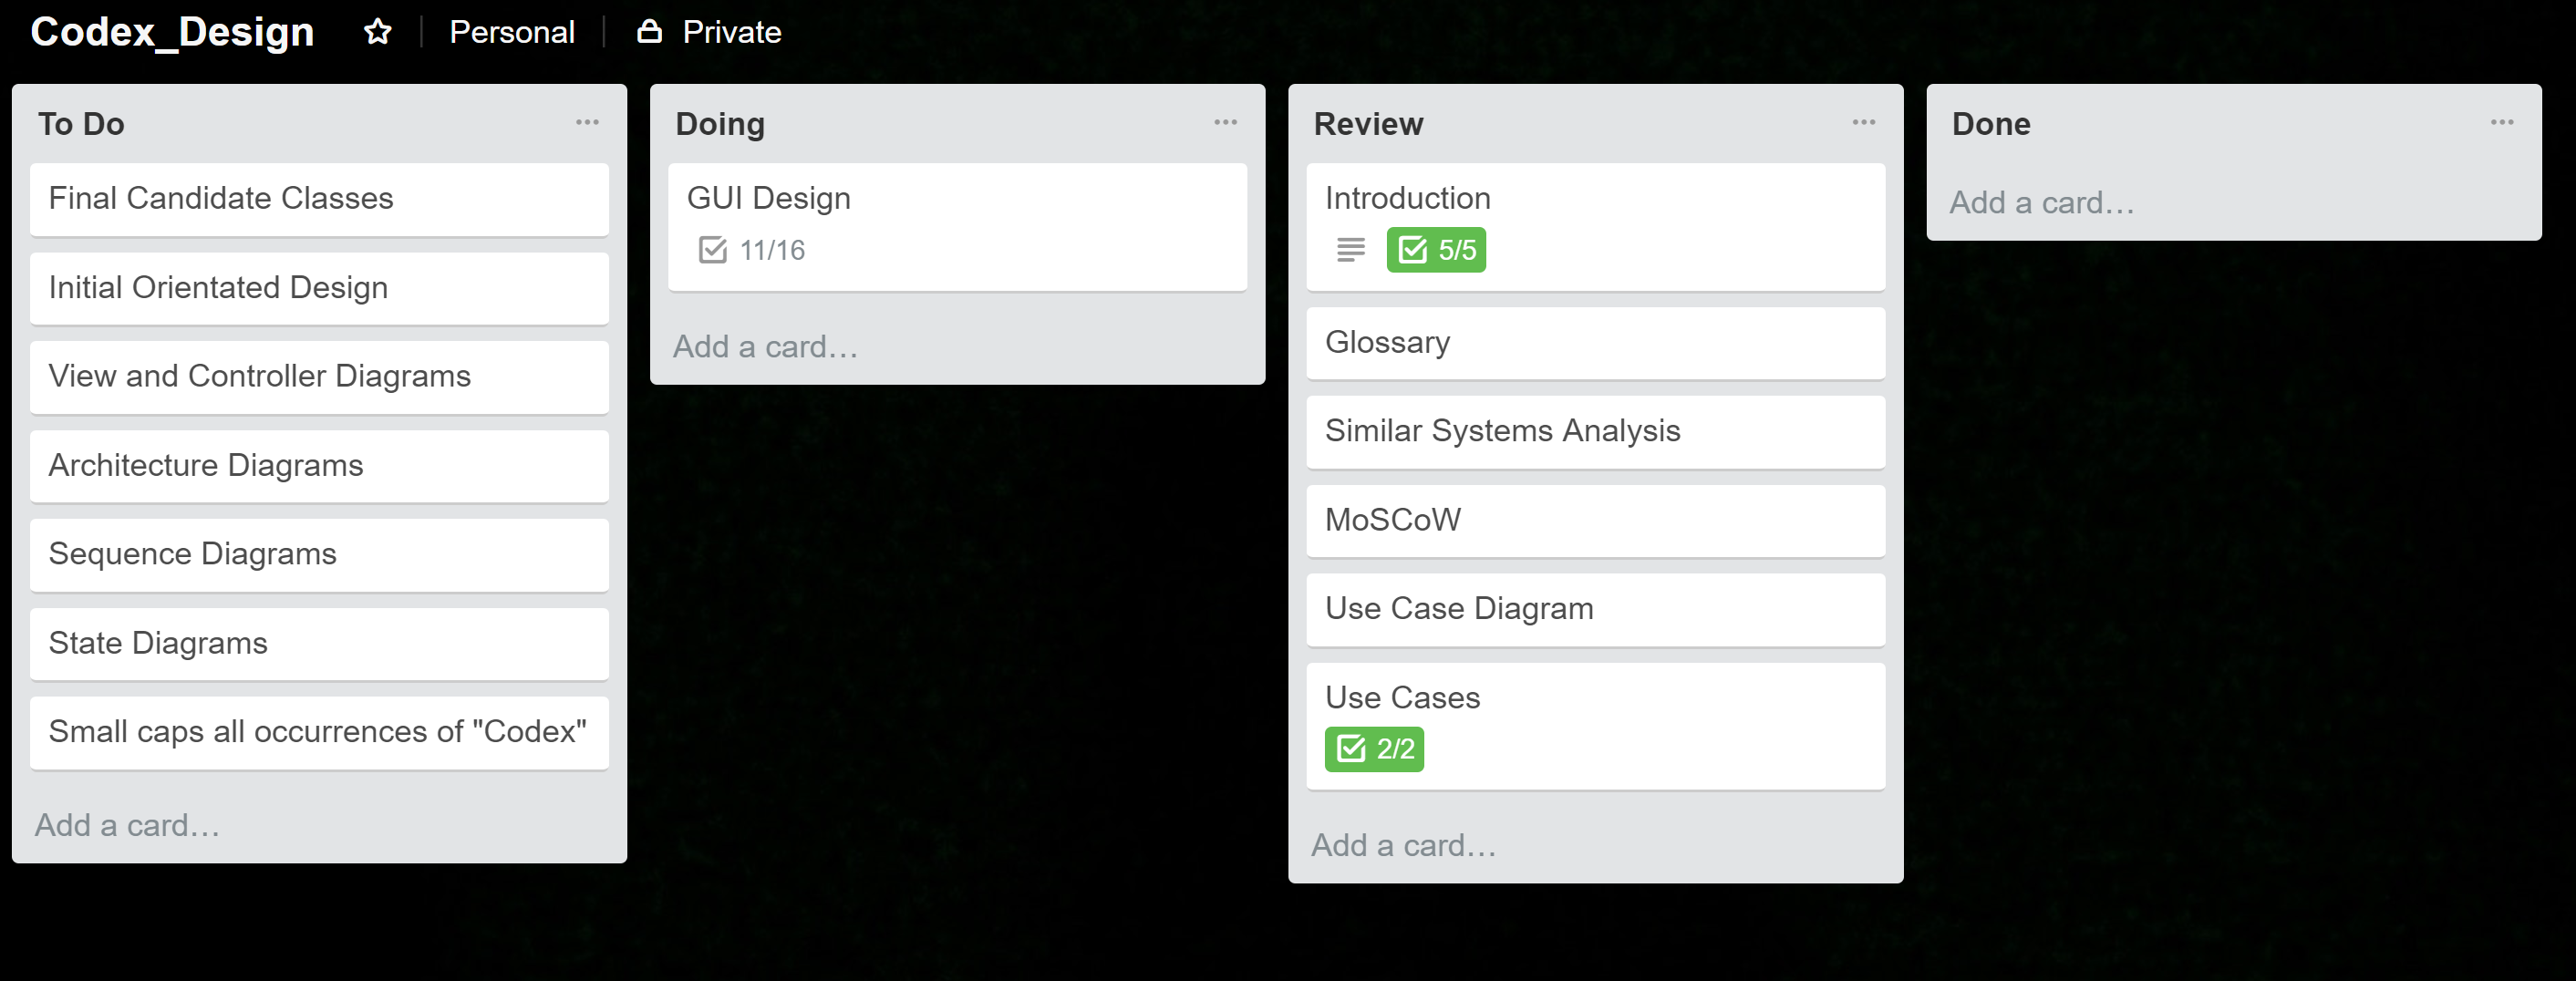
\includegraphics[width=0.5\textwidth]{trello_board.PNG}} 
		\caption{The Trello Board used to track the progress of the \Codex \ Design Iterations.} \label{fig:trello-board}
	\end{figure}
	
		\subsection{Iterative Design}
		\Codex \ has iterated through two design phases over the three months of development. The first phase focused on low fidelity (low-fi) prototyping of the User Interfaces and was designed with the use of PHP and ReactJS as its principle languages. However, to keep \Codex \ as simple as possible, PHP was replaced by Node.JS in the second iteration. This change was made in order to eliminate a set of testing to accommodate the use of a second language. Now \Codex \ development can be tested at every stage with a single set of testing classes. In addition to the change of language, the second iteration of \Codex \ Design focused on medium fidelity (mid-fi) prototyping of the GUI through the use of the Marvel App Website \citep{marvelapp}.
	
		\subsection{The Use of ReactJS and Node.JS}
		As discussed in section \ref{subsec:WIC}, \Codex \ aims to follow the Web-App Architecture. The \emph{presentation} and \emph{logic} tiers will be built using ReactJS with the communication to and from the \emph{data} tier will be written in Node.JS (with the database itself written in SQL). In addition to providing a clear separation of languages and functionality the three-tier Web-App Architecture also follows the Model-View-Controller (MVC) architectural pattern \citep{ModelViewController}. However, the MVC architecture is complicated by the use of ReactJS, which blurs the line between the \emph{Model} (logic) and \emph{View} (presentation) tiers. This is a problem that will be addressed in Section \ref{sec:Issues}.
		
		\subsection{\Codex \ System Requirements}
		The requirements for \Codex \ were generated by identifying the features that would solve the problems with \dnd \ that were discussed in Section \ref{sec:intro}. Once the features were generated, a \emph{MoSCoW Analysis} was performed on the list. The MoSCoW Analysis asks the developer which features \emph{must exist} in order for the system to be functional, then what \emph{should} be in the system in order to make it viable in the market. Once those two lists have been defined what \emph{could} the system posses that would be a nice addition to the other features. Finally MoSCoW asks what \emph{will not} be in the system at any point.
		\begin{landscape}
			\begin{table}
				\centering
				\caption{MoSCoW analysis for \Codex, showing the differing importance of wanted features to the system as a whole.}
				\label{tab:MoSCoW}
				\begin{tabular}{|l|l|l|l|}
					\hline
					\textbf{Must have} 					& \textbf{Should have}              & \textbf{Could have} & \textbf{Wont have}             \\ \hhline{|=|=|=|=|}
					Track Combat      					& Multiple Campaigns per DM Account	& Game Scheduling     & Full descriptions of D\&D      \\ \hline
					Accounts          					& Settings							& Items               & Pre-made Settings \& Campaigns \\ \hline
					Encounter Planning 					& Characters                        &                     & Inter-account Direct Messaging \\ \hline
					Random Encounters  					& WorldWiki                        	&                     &                                \\ \hline
					Populated Database 					& Run, Save \& Delete Games 		&                     &                                \\ \hline
					Session Planning					&         							&                     &                                \\ \hline
				\end{tabular}
			\end{table}
		\end{landscape}
	
		\subsection{Use Cases}
		Another critical part of the Design of \Codex \ is planning how the functionality of the system will flow. Use Cases and the Use Case Diagram inform a developer how a data is expected to flow between systems during a function. See Figure \ref{fig:use-case-diag} for the \Codex \ Use Case Diagram. This creates a road map for the development of a system to follow, increasing the speed of development due to the fact that developers already know what is expected of each function. At this current time, \Codex \ has 25 Use Cases. Minor functionality such as changing screens and submitting a form does not have their own Use Case, but are included in related Use Cases. 
		
		\begin{figure}
			\centering
			\fbox{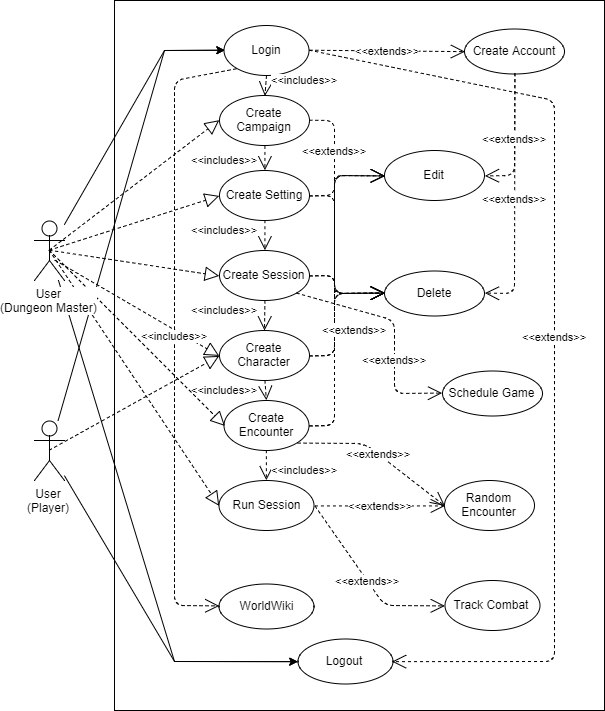
\includegraphics[width=0.5\textwidth]{use_case_diag.PNG}} 
			\caption{\Codex \ Use Case Diagram showing the accessibility to functions and the flow of information between them} \label{fig:use-case-diag}
		\end{figure}
	
		\begin{figure}
			\centering
			\fbox{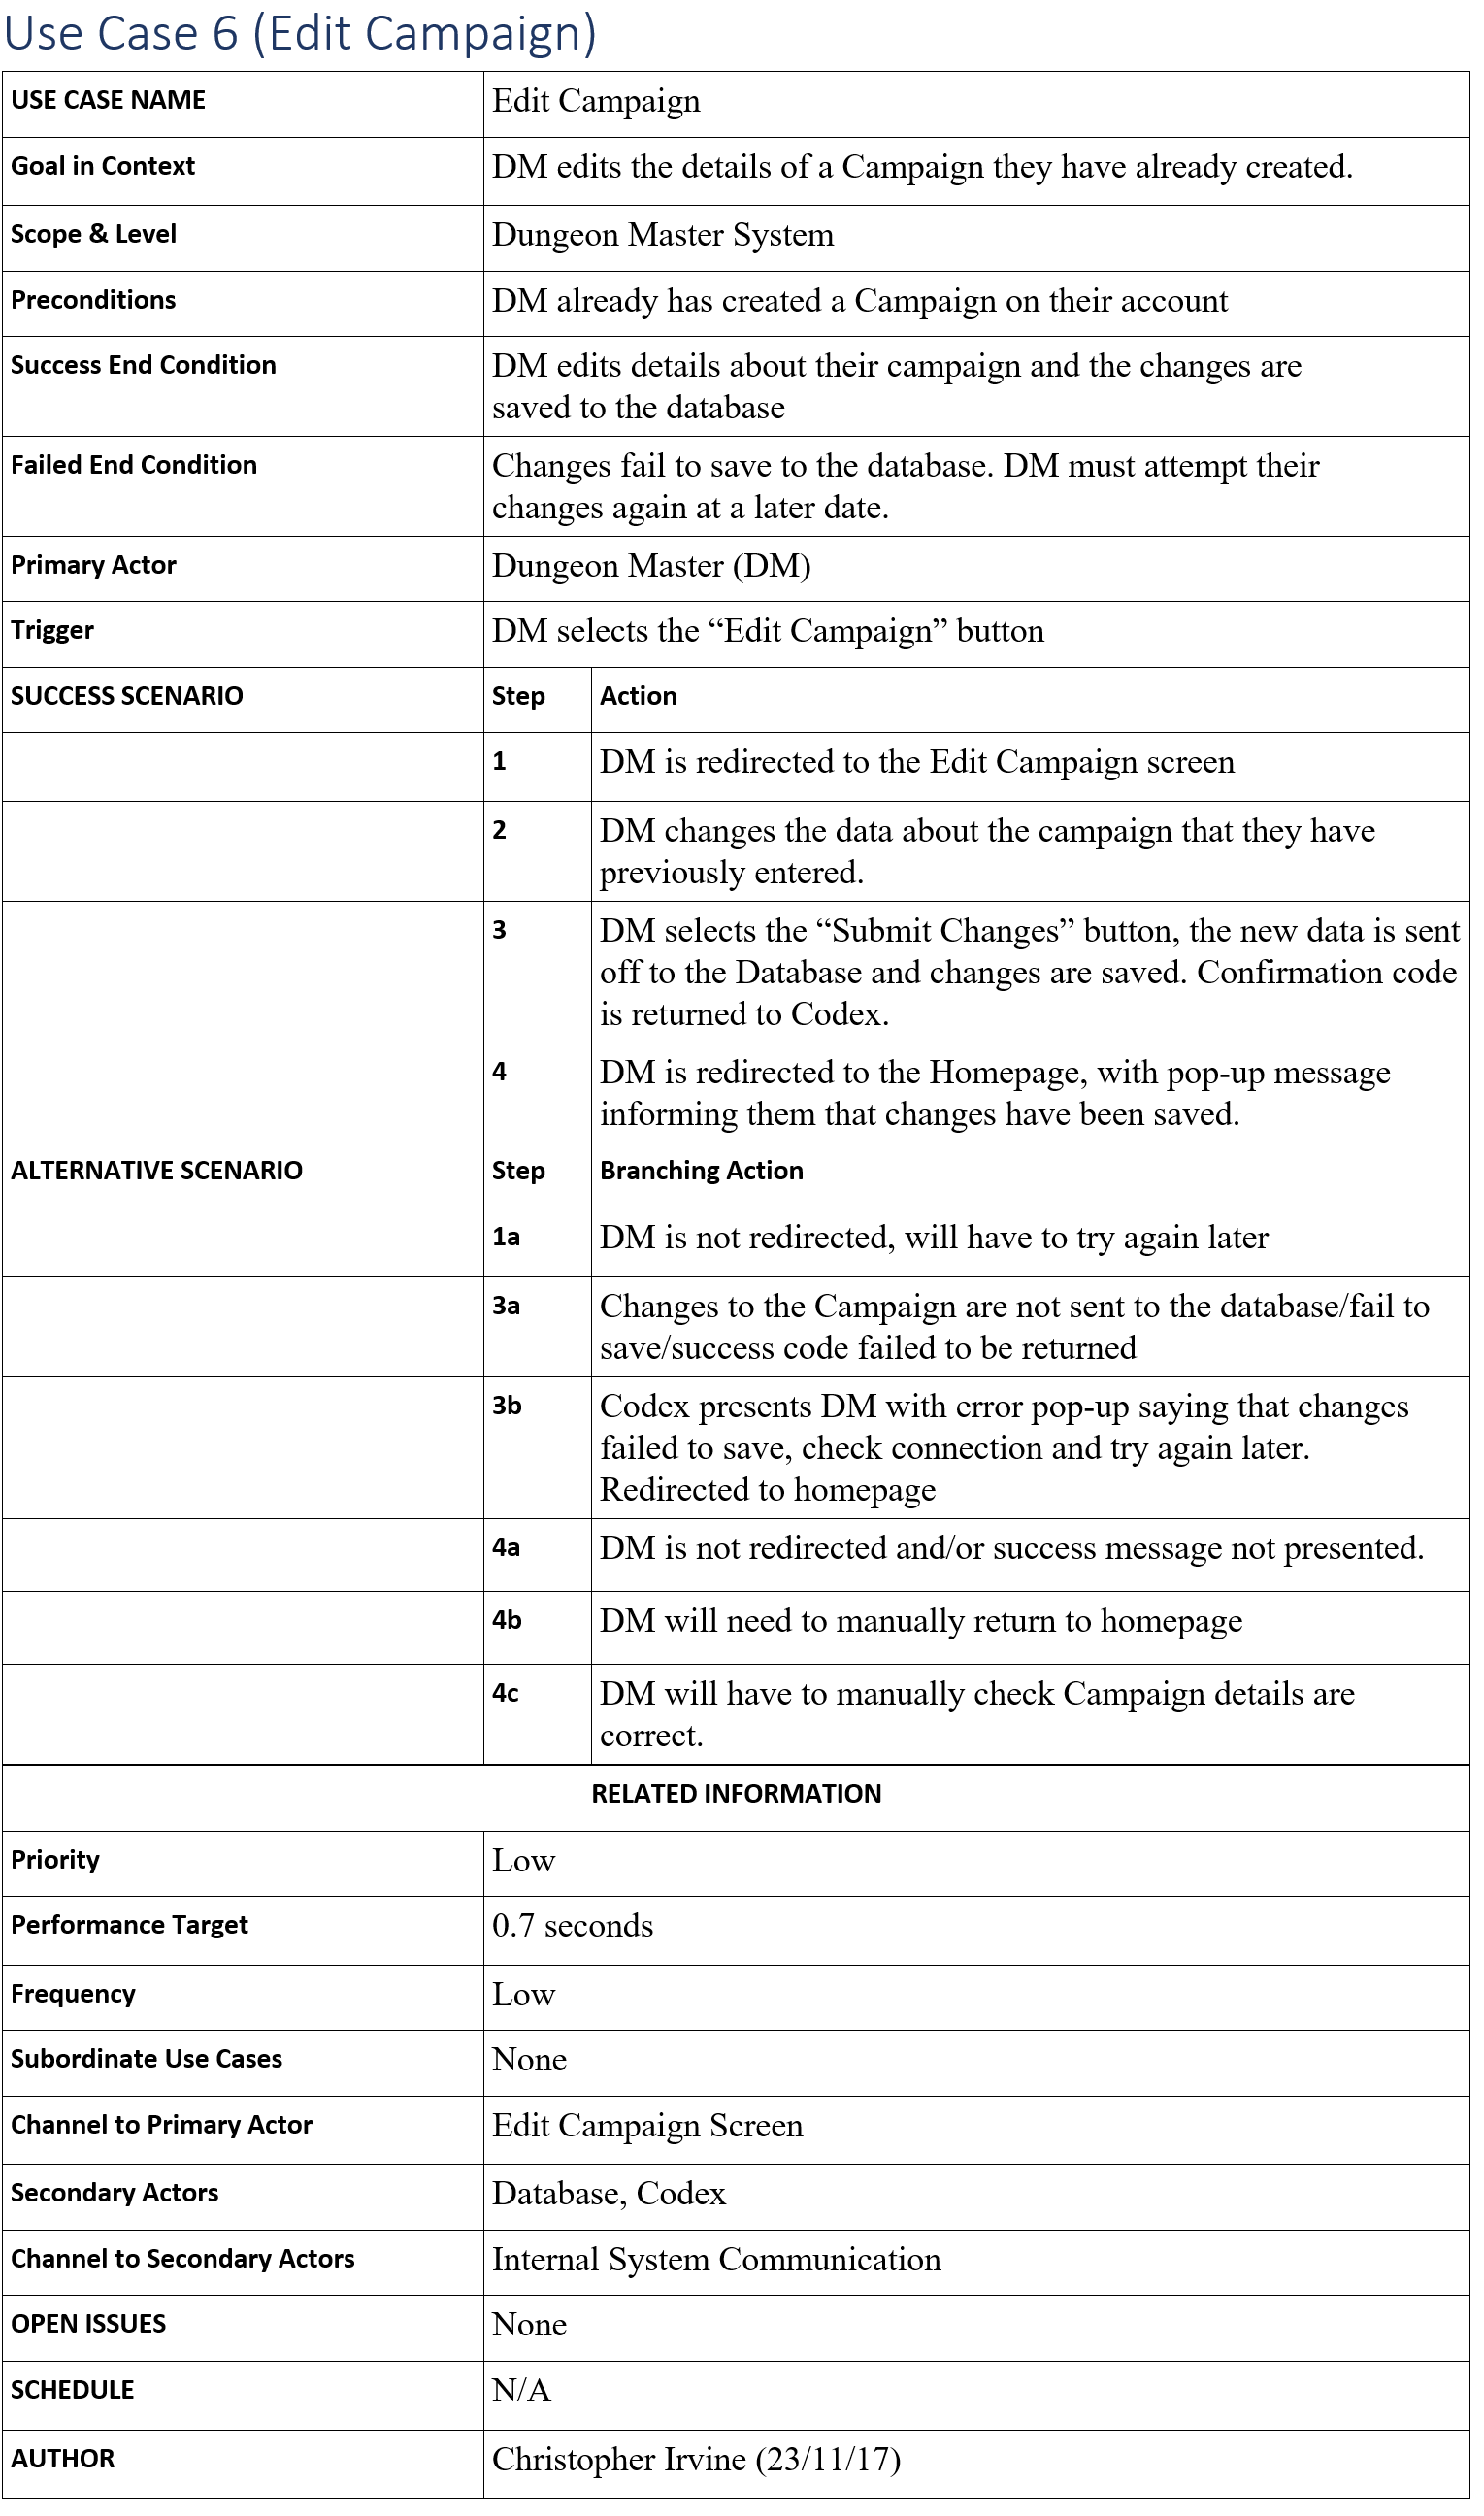
\includegraphics[width=0.75\textwidth]{use_case.PNG}}
			\caption{The Use Case for Editing an existing Campaign within \Codex}\label{fig:use-case}	
		\end{figure}
	
		\subsection{Low-Fi Prototyping}
		Discuss:
		\begin{itemize}
			\item What is Low-Fi
			\item Purpose of Low-Fi
			\item Think-Aloud Evaluations \& Results
			\item Changes to GUI made because of Think-Aloud
		\end{itemize}
	
		\subsection{Med-Fi Prototyping}
		Show the current med-fi prototypes built using MarvelApp.
		
		\subsection{Object Orientated Design}
		Discuss:
		\begin{itemize}
			\item What is OOD?
			\item What is the purpose of an OOD Diagram?
			\item Show the OOD Diagram for \Codex
		\end{itemize}
	
	\section{\Codex \ Implementation Plan}
	% How will the design be implemented?
	Discuss:
	\begin{itemize}
		\item Recap the Design Section that is directly related to Implementation (i.e. Choice of Languages/Architecture/OOD)
		\item Link to new Gantt Chart (see Appendix \ref{gc:new})
		\item Show command line modelling for combat? Screenshot of outputs?
		\item Reiterate Agile Solo
	\end{itemize}
	
	\section{Outstanding Issues} \label{sec:Issues}
	% What are the issues with Codex? Are they being addressed? Any forthcoming issues? 
	Outstanding Issues:
	\begin{itemize}
		\item Coursework taking up more time than expected, a couple of lost development days
		\item Haven't addressed the questionnaire mentioned in the proposal, pushed back to Design 3 and Development 2
	\end{itemize}
		\subsection{Solutions}
		% How are the solutions with Codex being addressed? Mitigate potential future issues?
		\begin{itemize}
			\item already simplified the MVP to help with the coursework issue
			\item need to develop the questionnaire and run it through ethics approval, use Christmas break to start this process
		\end{itemize}
	\section{Conclusion}
	% Summarise the progress that I have made, if it is enough and if not how can we do more?
	Discuss:
	\begin{itemize}
		\item overall happy with the current development of \Codex
			\subitem 
		\item iterate the importance of holiday development time
		\item summarise the issues and solutions
	\end{itemize}

	\clearpage
	\appendix
	\section{Gantt Chart - Original}
	\begin{cmpfigure}{\Codex \ Gantt Chart, outlining the major tasks and deliverables\label{gc:original}}
		\begin{sideways}
			\newganttchartelement{voidbar}{
				voidbar/.style={draw=black, top color=black!25, bottom color=black!23
			}}
			\begin{ganttchart}[y unit chart = 0.86cm, y unit title = 0.86cm, x unit=0.45cm, vgrid, title label font=\scriptsize,
				canvas/.style={draw=black, dotted}]{1}{34}
				\gantttitle{Project schedule shown for e-vision week numbers
					and semester week numbers}{34} \\
				
				\gantttitlelist{8,...,41}{1}\\
				\gantttitlelist{1,...,12}{1} \gantttitle{CB}{4}
				\gantttitlelist{1,...,9}{1} \gantttitle{EB}{4}
				\gantttitlelist{10,...,14}{1}\\
				
				%The elements, bars and milestones, are identified as elem0, elem1, etc.
				\ganttbar{Project Proposal}{1}{2} \\        		%elem0  
				\ganttbar{Literature Review}{2}{5} \\      			%elem1 
				\ganttmilestone{Literature Review Finished}{5} \\	%elem2
				\ganttbar{Design Doc. Iteration 1}{4}{8} \\ 		%elem3
				\ganttbar{Development Iteration 1}{9}{11} \\		%elem4
				\ganttbar{Progress Report}{11}{12} 					%elem5
				\ganttmilestone{}{12} \\							%elem6
				\ganttbar{Development Iteration 2}{11}{12}  		%elem7
				%week 1 of semester 2 is the 17th week in schedule 
				\ganttvoidbar{}{13}{16} \\                     		%elem8
				\ganttbar{Final Report Writing 1}{17}{19} 	        %elem9
				\ganttmilestone{}{19} \\							%elem10
				\ganttbar{Design Doc. Iteration 2}{19}{20} \\      	%elem11
				\ganttbar{Development Iteration 3}{21}{26} \\		%elem12
				\ganttbar{Testing}{24}{26} \\						%elem13
				\ganttmilestone{Code Delivery}{26} \\       		%elem14
				\ganttbar{Final Report Writing 2}{27}{30} \\  		%elem15
				\ganttbar{Inspection preparation}{31}{34}   		%elem16
				
				\ganttlink{elem0}{elem1} \ganttlink{elem1}{elem2} \ganttlink{elem2}{elem3}
				\ganttlink{elem3}{elem4} \ganttlink{elem4}{elem5} \ganttlink{elem5}{elem6}
				\ganttlink{elem5}{elem7} \ganttlink{elem8}{elem9} \ganttlink{elem10}{elem11}
				\ganttlink{elem11}{elem12} \ganttlink{elem12}{elem13} 
				\ganttlink{elem13}{elem14} \ganttlink{elem14}{elem15}
				\ganttlink{elem15}{elem16}
			\end{ganttchart}
		\end{sideways}
	\end{cmpfigure}

	\section{Gantt Chart - New}
	\begin{cmpfigure}{\Codex \ Gantt Chart, outlining the major tasks and deliverables\label{gc:new}}
		\begin{sideways}
			\newganttchartelement{voidbar}{
				voidbar/.style={draw=black, top color=black!25, bottom color=black!23
			}}
			\begin{ganttchart}[y unit chart = 0.86cm, y unit title = 0.86cm, x unit=0.45cm, vgrid, title label font=\scriptsize,
				canvas/.style={draw=black, dotted}]{1}{34}
				\gantttitle{Project schedule shown for e-vision week numbers
					and semester week numbers}{34} \\
				
				\gantttitlelist{8,...,41}{1}\\
				\gantttitlelist{1,...,12}{1} \gantttitle{CB}{4}
				\gantttitlelist{1,...,9}{1} \gantttitle{EB}{4}
				\gantttitlelist{10,...,14}{1}\\
				
				%The elements, bars and milestones, are identified as elem0, elem1, etc.
				\ganttbar{Project Proposal}{1}{2} \\        		%elem0  
				\ganttbar{Literature Review}{2}{5} \\      			%elem1 
				\ganttmilestone{Literature Review Finished}{5} \\	%elem2
				\ganttbar{Design Doc. Iteration 1}{4}{8} \\ 		%elem3
				\ganttbar{Design Doc. Iteration 2}{9}{11} \\		%elem4
				\ganttbar{Progress Report}{11}{12} 					%elem5
				\ganttmilestone{}{12} \\							%elem6
				\ganttbar{Development Iteration 1}{13}{17} \\  		%elem7
				%week 1 of semester 2 is the 17th week in schedule 
				\ganttbar{Final Report Writing 1}{17}{19} 	        %elem8
				\ganttmilestone{}{19} \\							%elem9
				\ganttbar{Design Doc. Iteration 3}{19}{20} \\      	%elem10
				\ganttbar{Development Iteration 2}{21}{26} \\		%elem11
				\ganttbar{Testing}{24}{26} \\						%elem12
				\ganttmilestone{Code Delivery}{26} \\       		%elem13
				\ganttbar{Final Report Writing 2}{27}{30} \\  		%elem14
				\ganttbar{Inspection preparation}{31}{34}   		%elem15
				
				\ganttlink{elem0}{elem1} \ganttlink{elem1}{elem2} \ganttlink{elem2}{elem3}
				\ganttlink{elem3}{elem4} \ganttlink{elem4}{elem5} \ganttlink{elem5}{elem6}
				\ganttlink{elem5}{elem7} \ganttlink{elem7}{elem8} \ganttlink{elem9}{elem10}
				\ganttlink{elem10}{elem11} \ganttlink{elem11}{elem12} 
				\ganttlink{elem12}{elem13} \ganttlink{elem13}{elem14} 
				\ganttlink{elem14}{elem15}
			\end{ganttchart}
		\end{sideways}
	\end{cmpfigure}
	
\bibliography{projectbib}
\end{document}
% EOF Document